% This file is included by main.tex

\chapter{GPU Architecture and Performance}
\label{ch::chapter4}

\vspace{-1cm}

\section{How a GPU Works}

\subsection*{Context and Relevance}
Having explored the significant capabilities of CPUs, particularly in handling complex sequential tasks, it is evident that they excel in low-latency operations and intricate control flows. However, when it comes to massive parallelization, GPUs emerge as the superior choice. Their architecture, specifically designed to execute thousands of simultaneous operations, makes them indispensable for tasks requiring extensive parallel processing.

In the last decade, Graphics Processing Units (GPUs) have evolved from being exclusive components for rendering graphics to becoming key tools in High-Performance Computing (HPC) \cite{GPUfundamentals}. Technologies such as artificial intelligence, physical simulations, data analysis, and scientific computing leverage the massive parallel architecture of GPUs, offering significant acceleration compared to Central Processing Units (CPUs).

\subsection*{Differences between CPUs and GPUs}
CPUs and GPUs have architectural designs optimized for different tasks:

\begin{itemize}
    \item \textbf{CPU (Central Processing Unit):}
    \begin{itemize}
        \item Designed to handle complex and sequential tasks.
        \item Contains few cores (typically on the order of 10-100) highly optimized for single-thread performance.
        \item Especially efficient for operations requiring low latency and complex control flows.
    \end{itemize}
    \item \textbf{GPU (Graphics Processing Unit):}
    \begin{itemize}
        \item Designed to execute a large number of operations in parallel.
        \item Contains hundreds or thousands of simpler cores organized in massively parallel processing blocks.
        \item Ideal for tasks with high parallelization, such as matrix multiplication and vector processing.
    \end{itemize}
\end{itemize}

\subsection{Host-Device Communication}
GPUs operate in conjunction with a CPU (host) through a well-defined communication topology. This topology involves two primary components:

\begin{itemize}
    \item \textbf{Host:} Refers to the CPU and its system memory (RAM).
    \item \textbf{Device:} Represents the GPU, including its on-board memories (global, shared, etc.).
\end{itemize}

\vspace{-1em}

\begin{figure}[H]
    \centering
    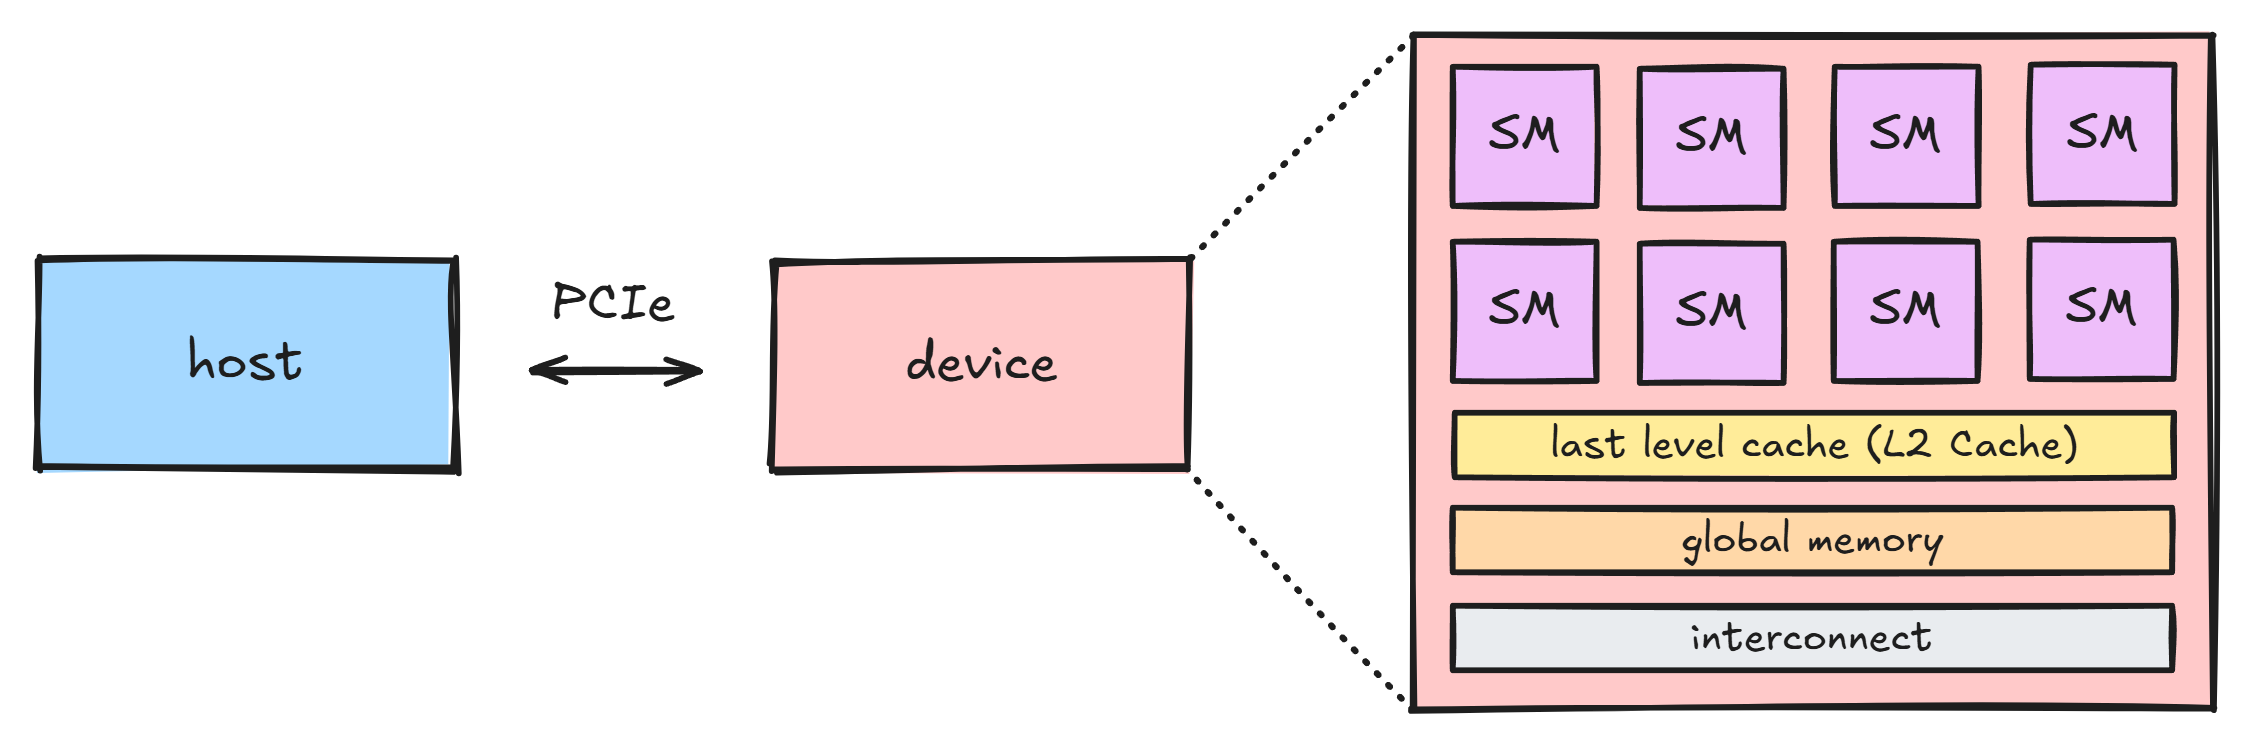
\includegraphics[width=0.8\textwidth]{figures/4_gpu/host_device_topology.png}
    \caption{Host-Device Communication Topology}
\end{figure}

\vspace{-0.5em}

This topology division is crucial as the code for launching the kernel and the data to be processed is also divided between a host function and a device function (kernel). The host is responsible for managing the data and launching the kernel, while the device executes the kernel in each thread and performs the computations.

A \textbf{kernel} \cite{GPUkerneloptimization,juliagpu} is a function that is executed by each thread in the GPU. The kernel must be written in a way that allows each thread to execute the same code but with different data. The host is responsible for launching the kernel to the GPU threads with the appropriate parameters and managing the data that will be processed by the kernel.

Before discussing the GPU itself, we need to understand that data transfer between the host and device occurs via the \textbf{PCI Express (PCIe) interface}.

\begin{table}[h]
    \centering
    \label{tab:pcie_bandwidth}
    \begin{tabular}{|c|c|c|c|c|}
        \hline
        \textbf{PCIe Version} & \textbf{Transfer Rate} & \textbf{x1 BW} & \textbf{x8 BW} & \textbf{x16 BW} \\
        \hline
        3.0 & 8 GT/s & 985 MB/s & 7.8 GB/s & 15.8 GB/s \\
        \hline
        4.0 & 16 GT/s & 1.97 GB/s & 15.8 GB/s & 31.5 GB/s \\
        \hline
        5.0 & 32 GT/s & 3.94 GB/s & 31.5 GB/s & 63 GB/s \\
        \hline
    \end{tabular}
    \caption{PCIe Bandwidth comparison for different versions.}
\end{table}

The NVIDIA GeForce RTX 3070 \cite{RTX3070specs} uses PCIe 4.0, achieving 31.5 GB/s maximum bandwidth for x16 connections. This typically isn't a bottleneck since data is usually transferred once at computation start and results returned at the end, but frequent host-device transfers could create bottlenecks.

\clearpage

\subsection{GPU Core Architecture and Memory}

The architecture of a GPU is designed to handle massive parallelization, with thousands of cores working simultaneously. The architecture is divided into several components, each with its own characteristics and functions.

\begin{figure}[H]
    \centering
    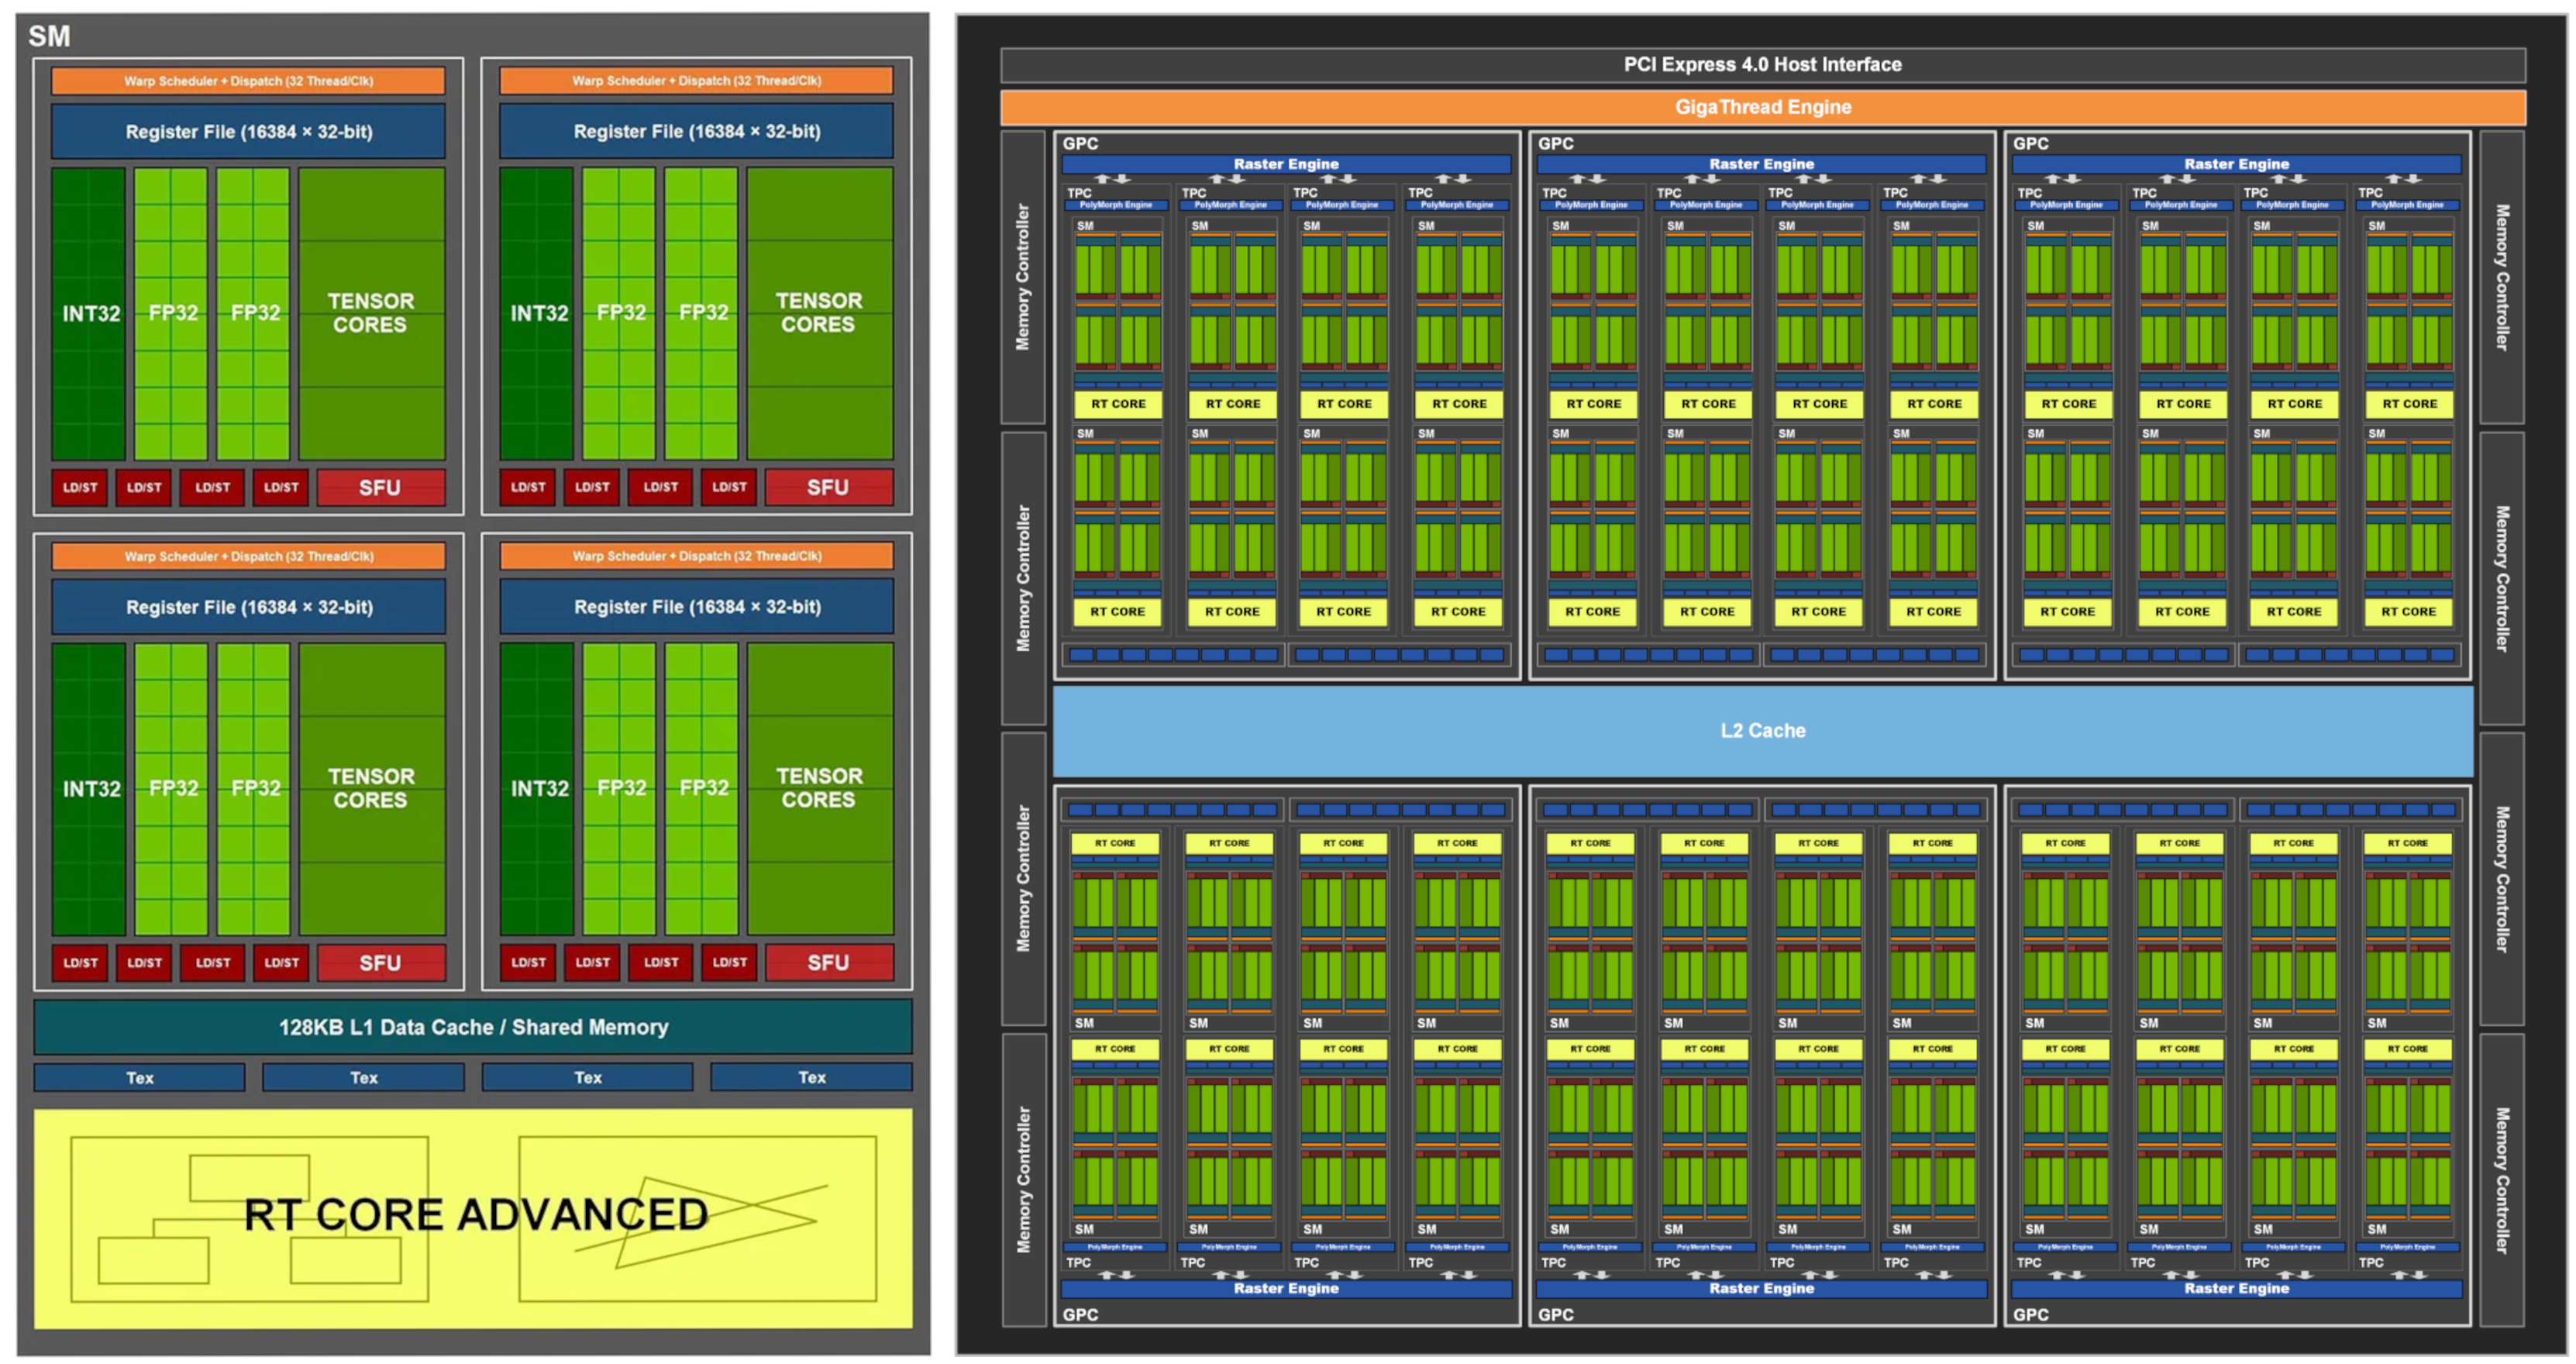
\includegraphics[height=8.5cm]{figures/4_gpu/GA104_Architecture.png}
    \caption{GA104 GPU (NVIDIA RTX 3070): Architecture and Streaming Multiprocessor}
\end{figure}

The GPU is divided into several Streaming Multiprocessors (SM), shown in the right image. AMD refers to these as Compute Units (CUs). Each SM contains several CUDA cores, which are the processing units of the GPU, responsible for executing threads in parallel. The CUDA cores are organized into warps, blocks, and grids \cite{GPUblocksandgrids}, which are the basic units of parallel execution in the GPU. This organization is explained in more detail in the next section.

The GPU architecture features a memory hierarchy divided into two regions \cite{GPUmemory}.

\textbf{On-Chip Memories (Per Streaming Multiprocessor):}
These provide high-speed access but with limited capacity.

\begin{itemize}
    \item \textbf{Registers:} The lowest-latency storage, integrated directly with the cores; organized into 32 banks (32 x 32-bit) corresponding to warp threads.
    \item \textbf{L1 Cache:} Serves as a buffer for register spills and frequently accessed data; physically unified with shared memory.
    \item \textbf{Shared Memory:} Explicitly managed by the programmer for intra-block data sharing; configurable partitioning with L1 cache.
    \item \textbf{Constant Caches:} Dedicated to read-only constants across threads in a warp or block.
\end{itemize}

\clearpage

\textbf{Off-Chip Memories (Shared Across Streaming Multiprocessors):}
These offer greater capacity at the expense of increased latency.

\begin{itemize}
    \item \textbf{L2 Cache:} A unified cache facilitating data transfer between global memory and PCIe.
    \item \textbf{Global Memory:} The primary device memory (e.g., GDDR6 on RTX 3070, bandwidth of approximately 500 GB/s); characterized by high latency (300--600 cycles).
    \item \textbf{Local Memory:} Utilized for register spill overflow beyond L1 and L2 caches; incurs significant performance penalties.
    \item \textbf{Texture and Constant Memory:} Optimized for specific access patterns, with texture data cached in L1 and constants in dedicated caches.
\end{itemize}

\subsubsection*{Memory Hierarchy}

The memory hierarchy in GPUs operates on principles of locality, both temporal (reusing data recently accessed) and spatial (accessing contiguous data), to minimize latency and maximize bandwidth in parallel workloads. When a thread requests data, the GPU traverses the hierarchy starting from the fastest, lowest-capacity levels closest to the cores, falling back to slower, higher-capacity levels only on misses.

\textbf{Data flow begins with registers}: if the required operand is in a thread's private registers, access is immediate (sub-cycle latency). \textbf{On a miss or overflow, the system checks the L1 cache} \cite{CPUcacheL1} (or shared memory for explicitly managed data), which may hit if the data was recently spilled or shared within the block. \textbf{Constant caches are consulted in parallel for read-only broadcasts}, optimizing uniform accesses across warps.

\textbf{If unresolved on-chip, the request propagates to the L2 cache} \cite{GPUcacheL2Global}, shared across SMs, which coalesces accesses from multiple warps and buffers global memory traffic. An L2 hit returns data in tens of cycles; \textbf{a miss triggers a fetch from global memory (DRAM)}.


\subsubsection*{Memory Locality}

Memory accesses in GPUs must be \textbf{coalesced} for efficiency: threads in a warp should access contiguous memory locations to minimize transactions. Non-coalesced accesses lead to serialized loads, wasting bandwidth.

In shared memory, \textbf{bank conflicts} occur when multiple threads access the same bank simultaneously, serializing accesses. Shared memory is divided into 32 banks (matching warp size), and proper padding or transposition can mitigate conflicts.

For global memory, alignment to 128-byte segments (cache line equivalent) is critical. In matrix operations, row-major versus column-major access patterns can cause uncoalesced loads, similar to CPU cache thrashing.

\subsubsection*{Tiling}

GPUs use \textbf{tiling} (also known as blocking in CPUs) to optimize performance by exploiting data locality. This technique involves loading small chunks of data, called tiles, from the slow global memory into the fast shared memory, where they can be reused multiple times by threads. This reduces the number of costly global memory accesses and increases \textbf{arithmetic intensity}, which measures the number of computations performed per byte of data transferred.

In a naive matrix multiplication, each thread computes one element of the result matrix \( C \), reading an entire row from matrix \( A \) and an entire column from matrix \( B \) from global memory. This leads to high memory traffic, roughly \( O(N^2) \) per thread, with low arithmetic intensity since few computations are done per data read. In contrast, tiling divides the matrices into smaller blocks, such as \( 32 \times 32 \) tiles, that fit in shared memory. Threads within a block work together to load these tiles, perform computations, and synchronize.

Libraries like \texttt{cuBLAS} and custom kernels apply \textbf{multi-level tiling}, using different tile sizes to optimize for shared memory, L1/L2 caches, and registers, depending on the GPU's architecture. For matrix-vector multiplication (MxV), however, tiling is less effective. Since each output element requires a full row of the matrix and the input vector with minimal data reuse, the operation has low arithmetic intensity (\( O(1) \)) and remains \textbf{bandwidth-bound}.

\subsection{Instruction-Level Parallelism: SIMT and Vectorization}

Modern GPUs employ a \textbf{Single Instruction, Multiple Threads (SIMT)} paradigm, analogous to SIMD in CPUs but scaled to thousands of threads. In SIMT, a single instruction is executed across multiple threads simultaneously, each operating on different data elements, making it highly efficient for data-parallel workloads like matrix operations.

Threads are grouped into \textbf{warps} (typically 32 threads on NVIDIA GPUs), executing the same instruction in lockstep. If threads in a warp diverge (e.g., due to conditional branching), the GPU serializes divergent paths, masking inactive threads, which can reduce efficiency. To maximize performance, kernels should minimize branch divergence.

FMA operations are critical in numerical workloads, counting as two floating-point operations per cycle. For matrix multiplication, high-level operations like GEMM are decomposed into tiled kernels that leverage SIMT parallelism and Tensor Cores for acceleration.

\clearpage

\section{Benchmarking on GPU}

In this section, we benchmark and compare the performance of \textbf{matrix–matrix multiplication} (MxM) and \textbf{matrix–vector multiplication} (MxV) on the GPU. The aim is to measure, for each operation, the sustained performance in $GFLOPS$ as the matrix size $N$ increases, and to contrast these measurements with theoretical limits imposed by both computation and memory access.

\vspace{0.5em}

\subsection*{Theoretical Compute Performance}

The theoretical time required to execute a given number of floating–point operations, assuming the GPU operates at its peak throughput, can be estimated as:

\begin{equation}
t_{GPU} = \frac{N_{ops}}{GFLOPS \times 10^9} \times 10^6,
\end{equation}

where $t_{GPU}$ is in microseconds.

The peak performance in $GFLOPS$ is computed as:

\begin{equation}
GFLOPS = C_{SM} \times C_{cores/SM} \times GPU_{GHz} \times M_{ops}.
\end{equation}

\noindent The terms in the equation are:
\begin{itemize}
    \item $C_{SM}$: number of Streaming Multiprocessors (e.g., 46 on RTX 3070).
    \item $C_{cores/SM}$: number of CUDA cores per SM (e.g., 128 on Ampere architecture).
    \item $GPU_{GHz}$: GPU clock speed in GHz (boost clock, e.g., 1.725 GHz on RTX 3070).
    \item $M_{ops}$: floating–point operations per cycle per core. For Fused Multiply–Add (FMA) instructions, each operation performs one multiplication and one addition in a single step, counting as two floating–point operations. On the NVIDIA RTX 3070 (Ampere), each CUDA core can execute 1 FMA per cycle, resulting in $M_{ops} = 2$.
\end{itemize}

This formula gives the peak for FP32 operations (e.g., 20.31 TFLOPS on RTX 3070). For FP64 in consumer GPUs, performance is typically limited intentionally (e.g., to 1/64 of FP32 on Ampere consumer cards, 317 GFLOPS) to encourage users needing high FP64 throughput to purchase more expensive HPC-oriented GPUs.

\clearpage

\subsection*{Theoretical Memory Access Performance}

Memory-bound operations are limited by global memory bandwidth or PCIe transfers. The time to access data is:

\begin{equation}
t_{mem} = \frac{N_{data} \times \text{Element Size}}{BW_{eff}} \times 10^6,
\end{equation}

where $BW_{eff}$ is the effective bandwidth and it is calculated dynamically from GPU attributes:

\begin{equation}
BW = 2 \times (f_{mem} \times 10^3) \times \frac{w_{bus}}{8},
\end{equation}

where:

\begin{itemize}
    \item $f_{mem}$ is the memory clock rate in kHz.
    \item $w_{bus}$ is the global memory bus width in bits.
    \item The factor $2$ accounts for double data rate (DDR) in GDDR memory.
    \item The $10^3$ converts kHz to Hz.
    \item Division by $8$ converts bits to bytes.
\end{itemize}

Both $f_{mem}$ and $w_{bus}$ can be obtained from the CUDA.jl package by running:

\begin{itemize}
    \item \texttt{CUDA.attribute(dev, CUDA.CU\_DEVICE\_ATTRIBUTE\_MEMORY\_CLOCK\_RATE)}
    \item \texttt{CUDA.attribute(dev, CUDA.CU\_DEVICE\_ATTRIBUTE\_GLOBAL\_MEMORY\_BUS\_WIDTH)}
\end{itemize}

This yields peak theoretical $BW$, e.g., $\approx 448 \times 10^9$ bytes/s (448 GB/s) on RTX 3070. 

For matrix-matrix multiplication (MxM), we estimate the real total memory access time by summing the individual measured components: the time to access a matrix by rows, the time to access a matrix by columns, and the time to allocate a matrix.

For matrix-vector multiplication (MxV), we sum the time to access a matrix by rows, the time to access a vector, and the time to allocate a vector.

\clearpage

\subsection{Benchmark Methodology}

The \textbf{GFLOPS benchmarks} are run using the \texttt{gflops\_1operation\_gpu.jl} script with CUDA.jl and cuBLAS. For each matrix size $N$, we do the following:
\begin{enumerate}
    \item Allocate random matrices/vectors on GPU: $A$ ($N \times N$), $B_{mat}$ ($N \times N$), $B_{vec}$ ($N \times 1$).
    \item Perform a warm-up multiplication to compile kernels.
    \item Benchmark a \textbf{single multiplication} using \texttt{@benchmark} (\texttt{evals=1}, 200 samples), taking the minimum time to compute sustained GFLOPS:
    \[
    GFLOPS_{\mathrm{MxM}} = \frac{2 N^3}{t_{MxM}} \times 10^{-9}, \quad GFLOPS_{\mathrm{MxV}} = \frac{2 N^2}{t_{MxV}} \times 10^{-9}.
    \]
\end{enumerate}

Theoretical peaks are derived from GPU specs via \texttt{gpu\_info()}. Benchmarks exclude host-device transfers to focus on pure device performance.

\textbf{Theoretical memory access time $t_{mem}$ and compute time $t_{GPU}$ benchmarks} are run using the \texttt{tgpu\_tmemory\_GPU.jl} script. For each matrix size $N$ we do:
\begin{enumerate}
    \item Compute the \textbf{theoretical times}:
    \begin{itemize}
        \item theoretical $t_{GPU}$: using the total number of floating-point operations for MxM or MxV and the peak $GFLOPS$ reported by \texttt{gpu\_info()} (based on SM count, clock, and FMA throughput, including the device FP32{:}FP64 ratio).
        \item theoretical $t_{mem}$: using the number of data elements to load/store and the GPU global memory bandwidth.
    \end{itemize}
    \item Measure the \textbf{measured execution times}:
    \begin{itemize}
        \item measured $t_{GPU}$: using \texttt{@benchmark} on $A \times B_{\text{mat}}$ (MxM, cuBLAS) and on $A \times B_{\text{vec}}$ (MxV, cuBLAS), device-only (excluding host–device transfers).
        \item measured $t_{mem}$: using \texttt{@benchmark} on memory access patterns over matrices and vectors (row-wise, column-wise, and vector) and on allocations, mirroring the CPU methodology.
    \end{itemize}
\end{enumerate}

\vspace{1em}

\subsubsection*{Libraries and System (GPU)}

All benchmarks and plots are using \texttt{CUDA.jl} and cuBLAS. 

The device is an NVIDIA GeForce RTX 3070 (Ampere, GA104) with 46 SMs and 8\,GB GDDR6 on a 256-bit bus (with an effective bandwidth of approximately 448\,GB/s).

Theoretical peaks are $\sim$20.3\,TFLOPS (FP32) and $\sim$317\,GFLOPS (FP64) (FP32{:}FP64 $\approx 64{:}1$).

\clearpage

\subsection{Benchmark results: GFLOPS}
\label{sec:gpu_bench_results_GFLOPS}

This section organizes the GPU GFLOPS discussion around three ideas:
(A) FP32 MxM vs.\ MxV, (B) FP32 MxM vs.\ FP64 MxM (hardware FP64 ratio), and (C) FP64 MxM vs.\ MxV. Throughout, we focus on trends rather than exact values.

\subsubsection*{(A) FP32: \textnormal{MxM} vs.\ \textnormal{MxV}}
On the RTX~3070, FP32 MxM ramps up quickly with $N$ and settles into a high plateau. This is the classic compute-bound behavior where cuBLAS tiling exploits shared memory and the L2 cache, keeping SM pipelines busy with high reuse.

In contrast, FP32 MxV stays far below, almost despreciable compared to MxM, and grows only modestly as $N$ increases. Its arithmetic intensity is tiny, so additional threads mostly wait on GDDR traffic rather than issuing more useful FMAs; performance is governed by memory bandwidth rather than by SM throughput.

\begin{figure}[H]\centering
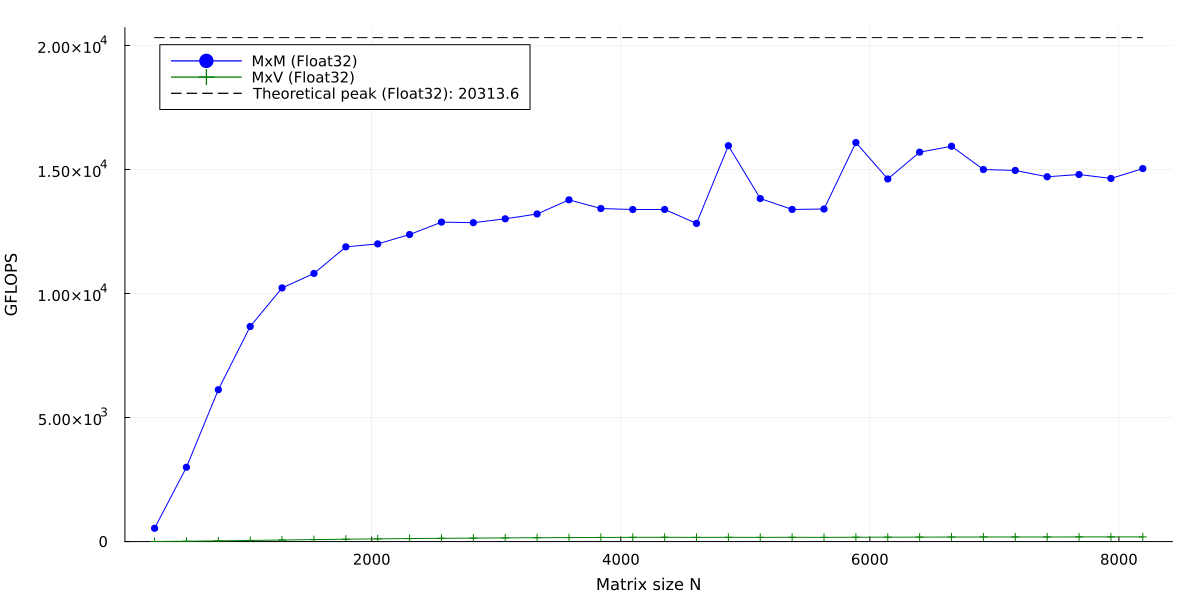
\includegraphics[width=\textwidth]{figures/4_gpu/gflops/FP32_GFLOPS_NVIDIA_GeForce_RTX_3070_MxM_vs_MxV.png}
\caption{\textbf{GFLOPS GPU FP32: MxM vs.\ MxV.} MxM, being compute-bound, climbs sharply and approaches a high plateau as cuBLAS tiles reuse data in shared memory and L2 cache. On the other hand, MxV, being memory-bound, sits much lower and changes little with $N$: extra parallelism cannot overcome the memory wall, so GFLOPS remain well below MxM.}
\label{fig:gpu_gflops_fp32_mxm_mxv}
\end{figure}

\noindent Minor undulations on the MxM curve at large $N$ are consistent with tile-size/occupancy boundaries and cache/L2 effects, but the overall picture remains a rise followed by a plateau.

\clearpage

\subsubsection*{(B) FP32 \textnormal{MxM} vs.\ FP64 \textnormal{MxM}}
Consumer Ampere GPUs throttle FP64 heavily (typically $\sim$1/64 of FP32 throughput). This is typically limited intentionally on consumer GPUs to encourage users needing high FP64 throughput to purchase more expensive HPC-oriented GPUs.

The result is that FP64 MxM reproduces the shape of the FP32 curve (tiling-driven ramp then plateau) but tops out at a much lower level, so cannot be even seen in the graph. This is fixed by a hardware ratio rather than by algorithmic limits. For large $N$, FP64 MxM consistently runs near its own (low) theoretical ceiling, illustrating that the bottleneck is architectural FP64 capacity, not inefficiency in the GEMM kernel.

\begin{figure}[H]\centering
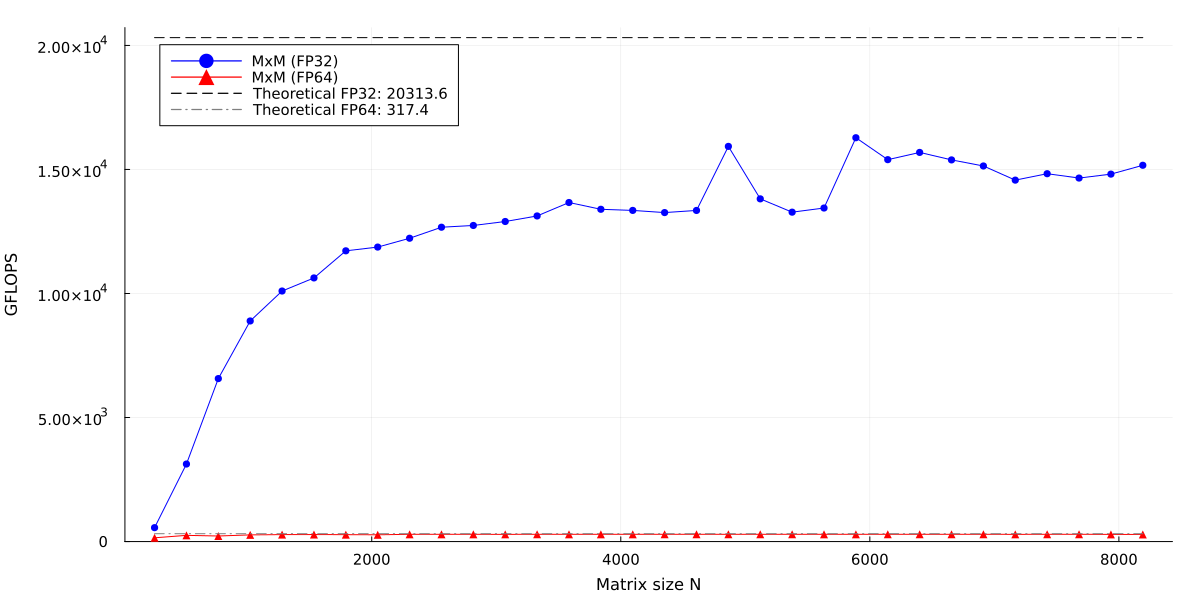
\includegraphics[width=\textwidth]{figures/4_gpu/gflops/FP32_vs_FP64_GFLOPS_NVIDIA_GeForce_RTX_3070_MxM.png}
\caption{\textbf{GFLOPS GPU: FP32 MxM vs.\ FP64 MxM.} Same scaling mechanics, different ceilings: FP64 saturates well below FP32 because consumer GPUs offer drastically reduced FP64 throughput. Large-$N$ FP64 MxM rides close to its own theoretical limit, highlighting a hardware cap rather than a software one.}
\label{fig:gpu_gflops_fp32_vs_fp64_mxm}
\end{figure}

The ratio between FP32 and FP64 units depends on the specific GPU architecture and its design choices.

For example, the NVIDIA RTX 3070 (Ampere consumer grade) has only 2 FP64 units per SM, while the NVIDIA A100 (a HPC grade oriented GPU) has 32 per SM.

\clearpage

\subsubsection*{(C) FP64: \textnormal{MxM} vs.\ \textnormal{MxV}}
With FP64, the MxM curve is compute-capped by the architecture as we commented earlier, and MxV remains bandwidth-bound. However, the GPU’s memory system is fast (the GPU NVIDIA RTX 3070 memory bandwidth is approximately 448 GB/s while the CPU’s is around 50 GB/s on DDR4 Dual Channel 3200 MHz).

Consequently, FP64 MxV climbs to a sizable fraction of FP64 MxM at large $N$ (much closer, in relative terms, than in FP32).

In other words, even though FP64 compute is throttled, the high GDDR bandwidth of the GPU lets a memory-bound kernel exploit a larger share of the available “budget” (the higher memory bandwidth) than it ever could on CPU RAM.

This is why FP64 MxV looks against FP32, comparatively healthy on the GPU, as the faster memory system provides a significant advantage.

\begin{figure}[H]\centering
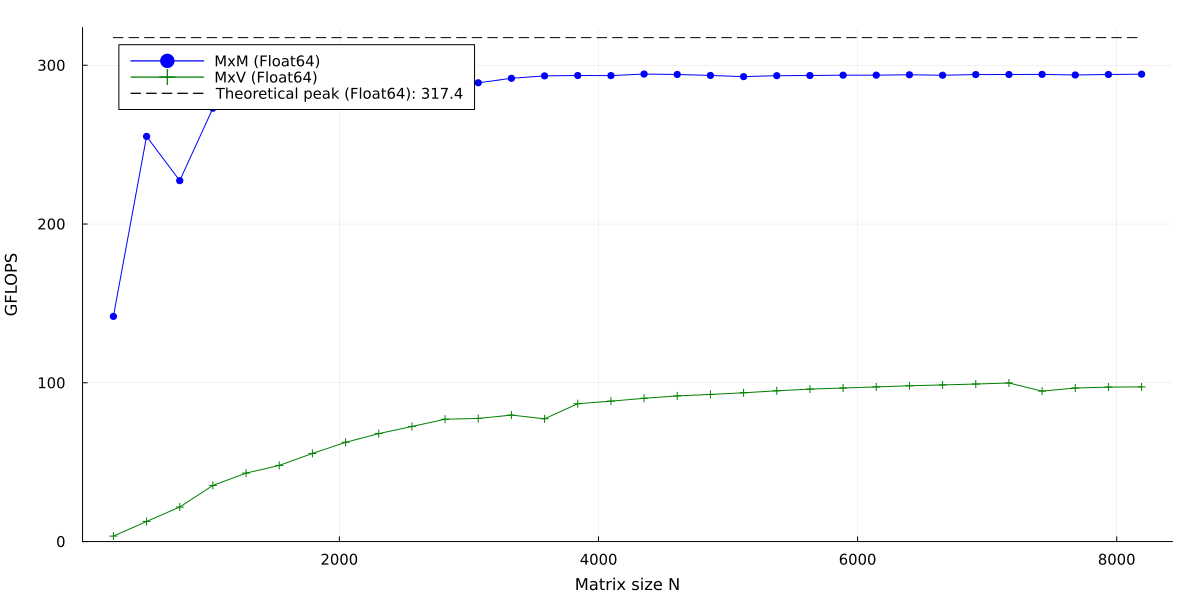
\includegraphics[width=\textwidth]{figures/4_gpu/gflops/FP64_GFLOPS_NVIDIA_GeForce_RTX_3070_MxM_vs_MxV.png}
\caption{\textbf{GFLOPS GPU FP64: MxM vs.\ MxV.} FP64 compute is heavily throttled, but memory bandwidth is unchanged. As a result, FP64 \textbf{MxV} (bandwidth-bound) reaches a substantial fraction of FP64 \textbf{MxM}, shrinking the relative gap vs.\ FP32. This underscores that the limiter for MxV is memory, where GPUs enjoy a big advantage over CPUs.}
\label{fig:gpu_gflops_fp64_mxm_mxv}
\end{figure}

Finally, in both precisions you may notice lower GFLOPS at very small $N$, where those points are dominated by fixed kernel-launch and setup overheads before the workload is large enough to amortize them.

\clearpage

\subsection{Benchmark results: theoretical vs measured time}
\label{sec:gpu_bench_results_theoretical_vs_measured_time}

We compare theoretical GPU compute time ($t_{\text{GPU}}$) and theoretical memory time ($t_{\text{mem}}$) to measured times. As with CPUs, $t_{\text{GPU}}$ is a compute-bound lower bound (ideal SM utilization), and $t_{\text{mem}}$ is a bandwidth-bound lower bound (ideal coalescing, no overheads).

\subsubsection*{(A) FP32: $t_{\text{GPU}}$ vs.\ $t_{\text{mem}}$ in \textnormal{MxM}}
For FP32 \textbf{MxM}, the operation-to-data ratio dominates again: $O(N^3)$ work over $O(N^2)$ data. cuBLAS’s tiling packs blocks into shared memory, driving reuse and keeping warps busy; measured times follow $t_{\text{GPU}}$ closely and stay well above $t_{\text{mem}}$ for moderate/large $N$.

\begin{figure}[H]\centering
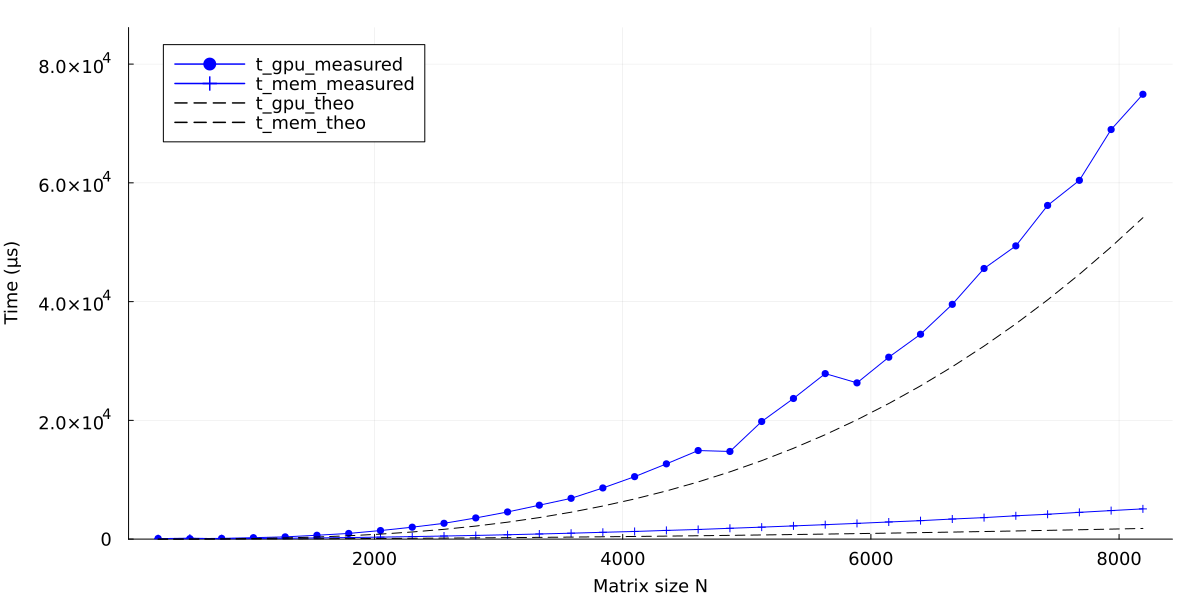
\includegraphics[width=\textwidth]{figures/4_gpu/tgpu_tmemory/Float32_MXM_NVIDIA_GeForce_RTX_3070.png}
\caption{\textbf{GPU FP32 MxM: theoretical vs.\ measured times.} Compute-bound: measured \(t_{\text{GPU}}\) tracks the theoretical \(t_{\text{GPU}}\) as tiling and reuse sustain high SM occupancy; \(t_{\text{mem}}\) remains a lower bound that is not reached in practice. The \(O(N^3)\) vs.\ \(O(N^2)\) scaling widens the gap with $N$.}
\label{fig:gpu_tgpu_tmem_fp32_mxm}
\end{figure}

We can observe that the measured time is consistently above the theoretical compute time, which is expected due to overheads and inefficiencies. However, the gap does not widen dramatically with $N$ because the kernel remains compute-bound, and cuBLAS optimizations keep the GPU busy.

\clearpage

\subsubsection*{(B) FP32 (low-$N$ zoom): kernel-launch overheads}
At small sizes, fixed costs dominate (kernel launch latency, queueing, synchronization, initializations). Both measured curves sit far above their theoretical bounds: there is simply too little work to amortize the launch.

\begin{figure}[H]\centering
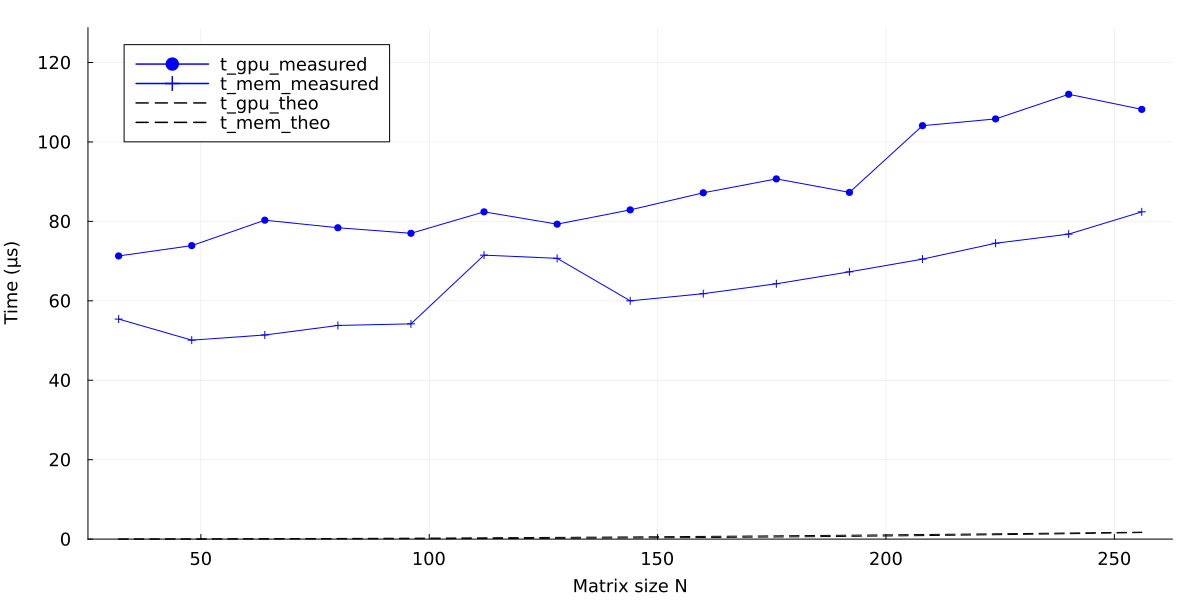
\includegraphics[width=\textwidth]{figures/4_gpu/tgpu_tmemory/Float32_MXM_NVIDIA_GeForce_RTX_3070_lowN.png}
\caption{\textbf{GPU FP32 MxM (low-$N$ zoom):} Measured times \(\gg\) theoretical bounds due to launch/scheduling overheads and underutilization of SMs at tiny problem sizes. Past a threshold $N$, overheads are amortized and the curve collapses toward the compute-bound regime.}
\label{fig:gpu_tgpu_tmem_fp32_mxm_lown}
\end{figure}

Concretely, at $N{=}32$ the theoretical times are essentially negligible (\(t_{\text{GPU}}\!\approx 0\,\mu\mathrm{s}\), \(t_{\text{mem}}\!\approx 0\,\mu\mathrm{s}\)), while the measurements are around the \(80\,\mu\mathrm{s}\) mark.

Even at $N{=}256$, the theoretical \(t_{\text{GPU}}\) does not match the measured \(t_{\text{GPU}}\!\approx 100\,\mu\mathrm{s}\). These gaps are the fixed launch/setup costs being amortized too slowly at small problem sizes.

This is due to the host-device model: the CPU must launch the kernel and manage data transfers, which adds latency that is significant when the workload is small.

\clearpage

\subsubsection*{(C) FP64: $t_{\text{GPU}}$ vs.\ $t_{\text{mem}}$ in \textnormal{MxM}}
In FP64 MxM the operation-to-data ratio still rules: $2N^3$ FLOPs vs.\ $\mathcal{O}(N^2)$ bytes.

However, as consumer GPUs throttle FP64 throughput (e.g., $\sim$1/32–1/64 of FP32), the kernel is even more compute-bound. As we see at the y-axis scale, the measured $t_{\text{GPU}}$ reaches two orders above that we had in FP32.

Again, $t_{\text{mem}}$ remains well below compute time despite doubling the element size (8\,B) relative to FP32.

\begin{figure}[H]\centering
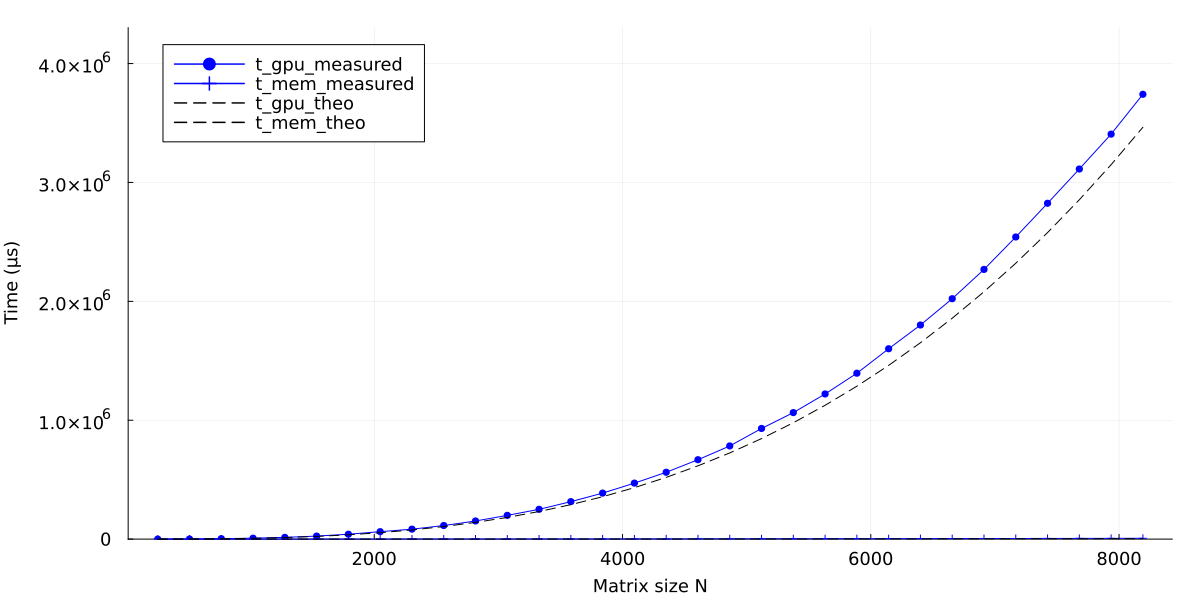
\includegraphics[width=\textwidth]{figures/4_gpu/tgpu_tmemory/Float64_MXM_NVIDIA_GeForce_RTX_3070.png}
\caption{\textbf{GPU FP64 MxM: theoretical vs.\ measured times.} Same $N^3$ vs.\ $N^2$ scaling, but FP64 throughput is hardware-limited on consumer GPUs. Memory traffic (now 8\,B per element) still scales as $\mathcal{O}(N^2)$ and stays below compute. The measured $t_{\text{GPU}}$ sits nearer its theoretical lower bound due to reduced memory bandwidth utilization and pressure.}
\label{fig:gpu_tgpu_tmem_fp64_mxm}
\end{figure}

Compute is artificially capped, but memory does not dominate anyway, and measured $t_{\text{GPU}}$ aligns more tightly with the ideal trend because of reduced memory bandwidth utilization. As a result, the measured $t_{\text{GPU}}$ lies closer to its theoretical curve (smaller gap) because memory pressure is even lower than in FP32.

